\scanpage{23}
\figure{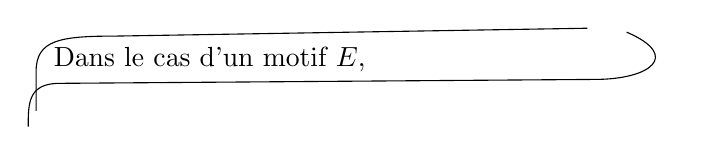
\begin{tikzpicture}[x=1cm,y=1cm]
\draw (0,0)--(0,0.5).. controls (0,0.9) and (0.3,0.95)..(1,0.95)--(7,1.05);\draw (7.5,1).. controls (8.2,0.7) and (7.8,0.4)..(7.1,0.4)--(0.3,0.35).. controls (-0.1,0.35) and (-0.1,0.1)..(-0.1,-0.2);
\node[anchor=west] at (0.1,0.65) {Dans le cas d'un \uline{motif} $E$,};
\end{tikzpicture}}
\unsure{Si} on exprime $\delta(E)$ et $\chi(E)$ en termes des \deleted{\unsure{ses}} composantes virtuelles de $\mathbf R f_!(E)$ (utilisant conj. de Weil), on trouve
\[
\left\{\begin{aligned}
\chi(E)&=\sum(-1)^i\beta_i(E)\\
\delta(E)&=\prod_i\delta(h_!^i(E))^{(-1)^i}
\end{aligned}\right.
\]
\margin{$\beta_i(E)$ les \unsure{nbs|nbres} de Betti virtuels à coeff. dans $E$}

Or $h_!^i(E)$ donne $\beta_i$ valeurs propres de val. absolue $p^{i/2}$, donc
\[\deleted{\unsure{\delta(E)=}}\delta(h_!^i(E))=\varepsilon_i p^{\frac{i\beta_i}{2}}\]
\margin{(NB. $i\beta_i/2$ : tjrs entier)}
où \deleted{$\unsure{\delta}$} $\varepsilon_i$ est défini comme un signe de discriminant virtuel, et c'est \deleted{$\unsure{\varepsilon}$} $+1$ si $i$ est impair. On trouve alors
\[
\left\{\begin{aligned}
\delta(E)&=\deleted{\unsure{\varepsilon(E)p^{\frac12\sum_i i\beta_i}}}\varepsilon(E)p^{\frac12\sum_i(-1)^i i\beta_i(E)}\\
\varepsilon(E)&=\prod_i\varepsilon_i(E)
\end{aligned}\right.
\]
\margin{$\varepsilon(E)$ et les $\varepsilon_i(E)$ sont $\pm1$, $\varepsilon_i(E)=+1$ si $i$ impair.}
\mspage{22}
